% Ubah judul dan label berikut sesuai dengan yang diinginkan.
\section{Pengujian dan Analisis}
\label{sec:PengujianAnalisa}

Pada penelitian ini dipaparkan hasil dari metodologi serta pembahasan analisis dari model dan implementasinya.

\subsection{Hasil Training dan Validation}
\label{sec:hasiltrainval}

\begin{enumerate}[nolistsep]

  \item Transfer Learning ResNet50 \\
  Lorem ipsum dolor sit amet, consectetur adipiscing elit, sed do eiusmod tempor incididunt ut labore et dolore magna 
  aliqua.

  \begin{figure} [ht]
    \centering
    % Ubah sesuai dengan nama file gambar dan ukuran yang akan digunakan.
    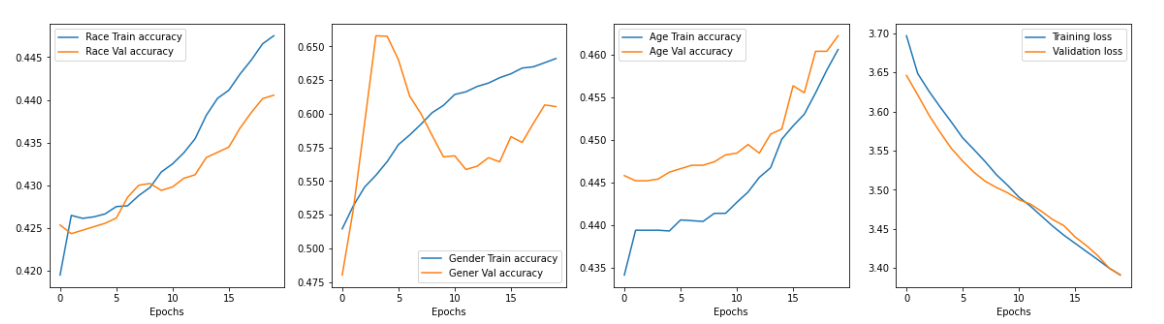
\includegraphics[width=0.5\textwidth]{gambar/PlotResNet50.png}

    % Ubah sesuai dengan keterangan gambar yang diinginkan.
    \caption{Plot Train dan Val ResNet50}
    \label{fig:PlotResNet50}
  \end{figure}

  \item Transfer Learning VGG16 \\
  Lorem ipsum dolor sit amet, consectetur adipiscing elit, sed do eiusmod tempor incididunt ut labore et dolore magna 
  aliqua.

  \begin{figure} [ht]
    \centering
    % Ubah sesuai dengan nama file gambar dan ukuran yang akan digunakan.
    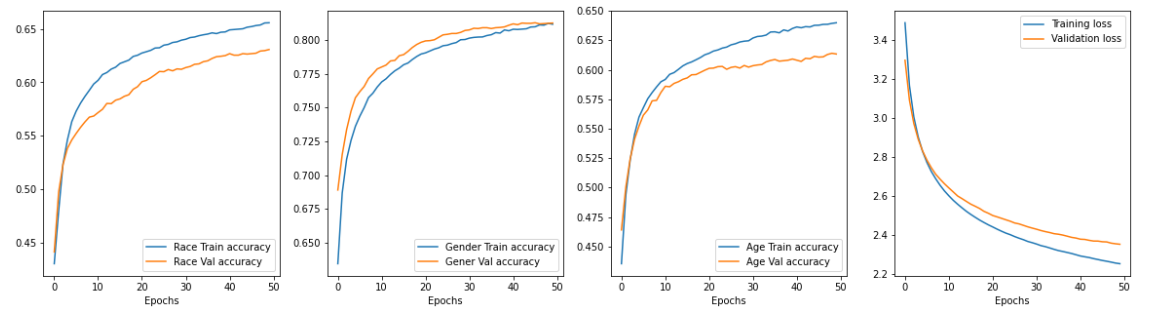
\includegraphics[width=0.5\textwidth]{gambar/PlotVGG16.png}

    % Ubah sesuai dengan keterangan gambar yang diinginkan.
    \caption{Plot Train dan Val VGG16}
    \label{fig:PlotVGG16}
  \end{figure}

  \item Transfer Learning EfficienNet B0 \\
  Lorem ipsum dolor sit amet, consectetur adipiscing elit, sed do eiusmod tempor incididunt ut labore et dolore magna 
  aliqua. \\

  \begin{figure} [ht]
    \centering
    % Ubah sesuai dengan nama file gambar dan ukuran yang akan digunakan.
    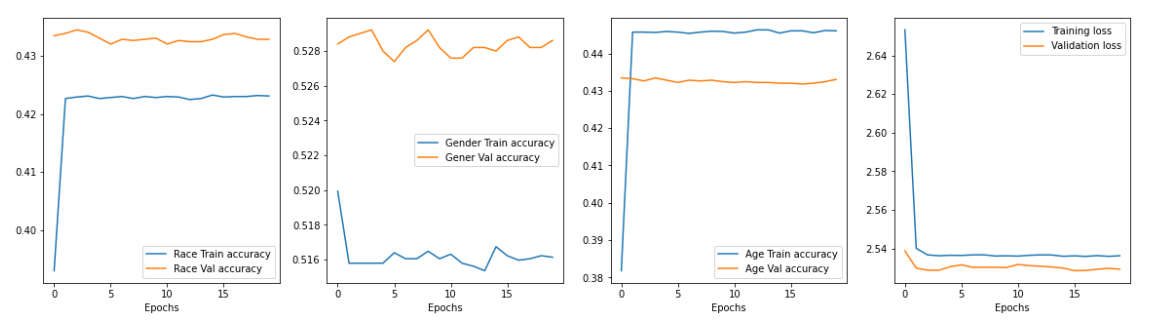
\includegraphics[width=0.5\textwidth]{gambar/PlotEfficienNet.png}

    % Ubah sesuai dengan keterangan gambar yang diinginkan.
    \caption{Plot Train dan Val EfficienNet B0}
    \label{fig:PlotEfficienNetB0}
  \end{figure}

  \item Transfer Learning Inception V3 \\
  Lorem ipsum dolor sit amet, consectetur adipiscing elit, sed do eiusmod tempor incididunt ut labore et dolore magna 
  aliqua. \\

  \begin{figure} [ht]
    \centering
    % Ubah sesuai dengan nama file gambar dan ukuran yang akan digunakan.
    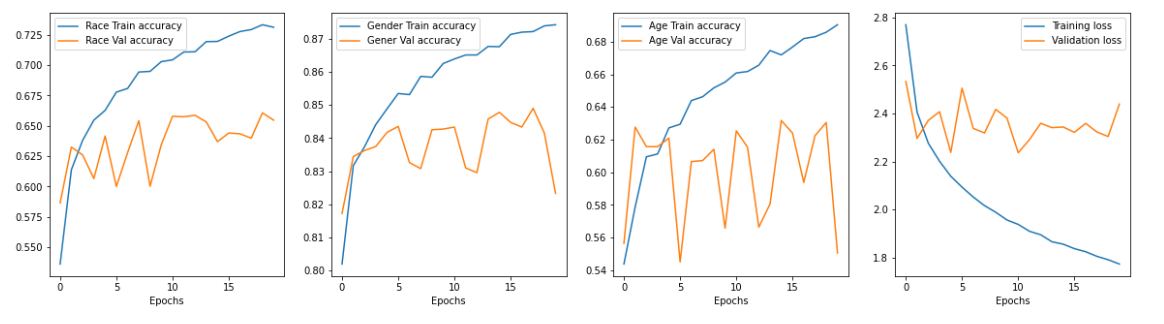
\includegraphics[width=0.5\textwidth]{gambar/PlotInceptionV3.png}

    % Ubah sesuai dengan keterangan gambar yang diinginkan.
    \caption{Plot Train dan Val Inception V3}
    \label{fig:PlotInceptionV3}
  \end{figure}

  \item Arsitektur CNN Sederhama \\
  Lorem ipsum dolor sit amet, consectetur adipiscing elit, sed do eiusmod tempor incididunt ut labore et dolore magna 
  aliqua. \\

  \begin{figure} [ht]
    \centering
    % Ubah sesuai dengan nama file gambar dan ukuran yang akan digunakan.
    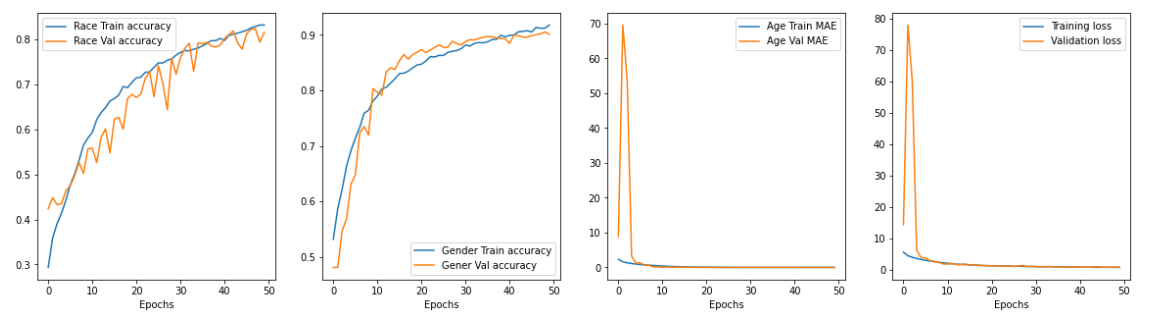
\includegraphics[width=0.5\textwidth]{gambar/PlotModel.png}

    % Ubah sesuai dengan keterangan gambar yang diinginkan.
    \caption{Plot Train dan Val Arsitektur CNN sederhana}
    \label{fig:PlotCNNSederhana}
  \end{figure}

\subsection{Hasil Testing Prototype Web}
\label{sec:hasiltestingprotoype}

  Untuk pengujian prototype sistem melalui web, hasil yang didapatkan dapat dilihat dari estimasi yang ditampilkan pada 
  web. Hasil prediksinya sangat dipengaruhi oleh pencahayaan pada foto, karena detail dari wajah bisa saja terutupi atau 
  dilebihkan. Berikut adalah hasil prediksi dari metode upload foto pada Gambar\ref{fig:upload}.

  \begin{figure} [ht]
    \centering
    % Ubah sesuai dengan nama file gambar dan ukuran yang akan digunakan.
    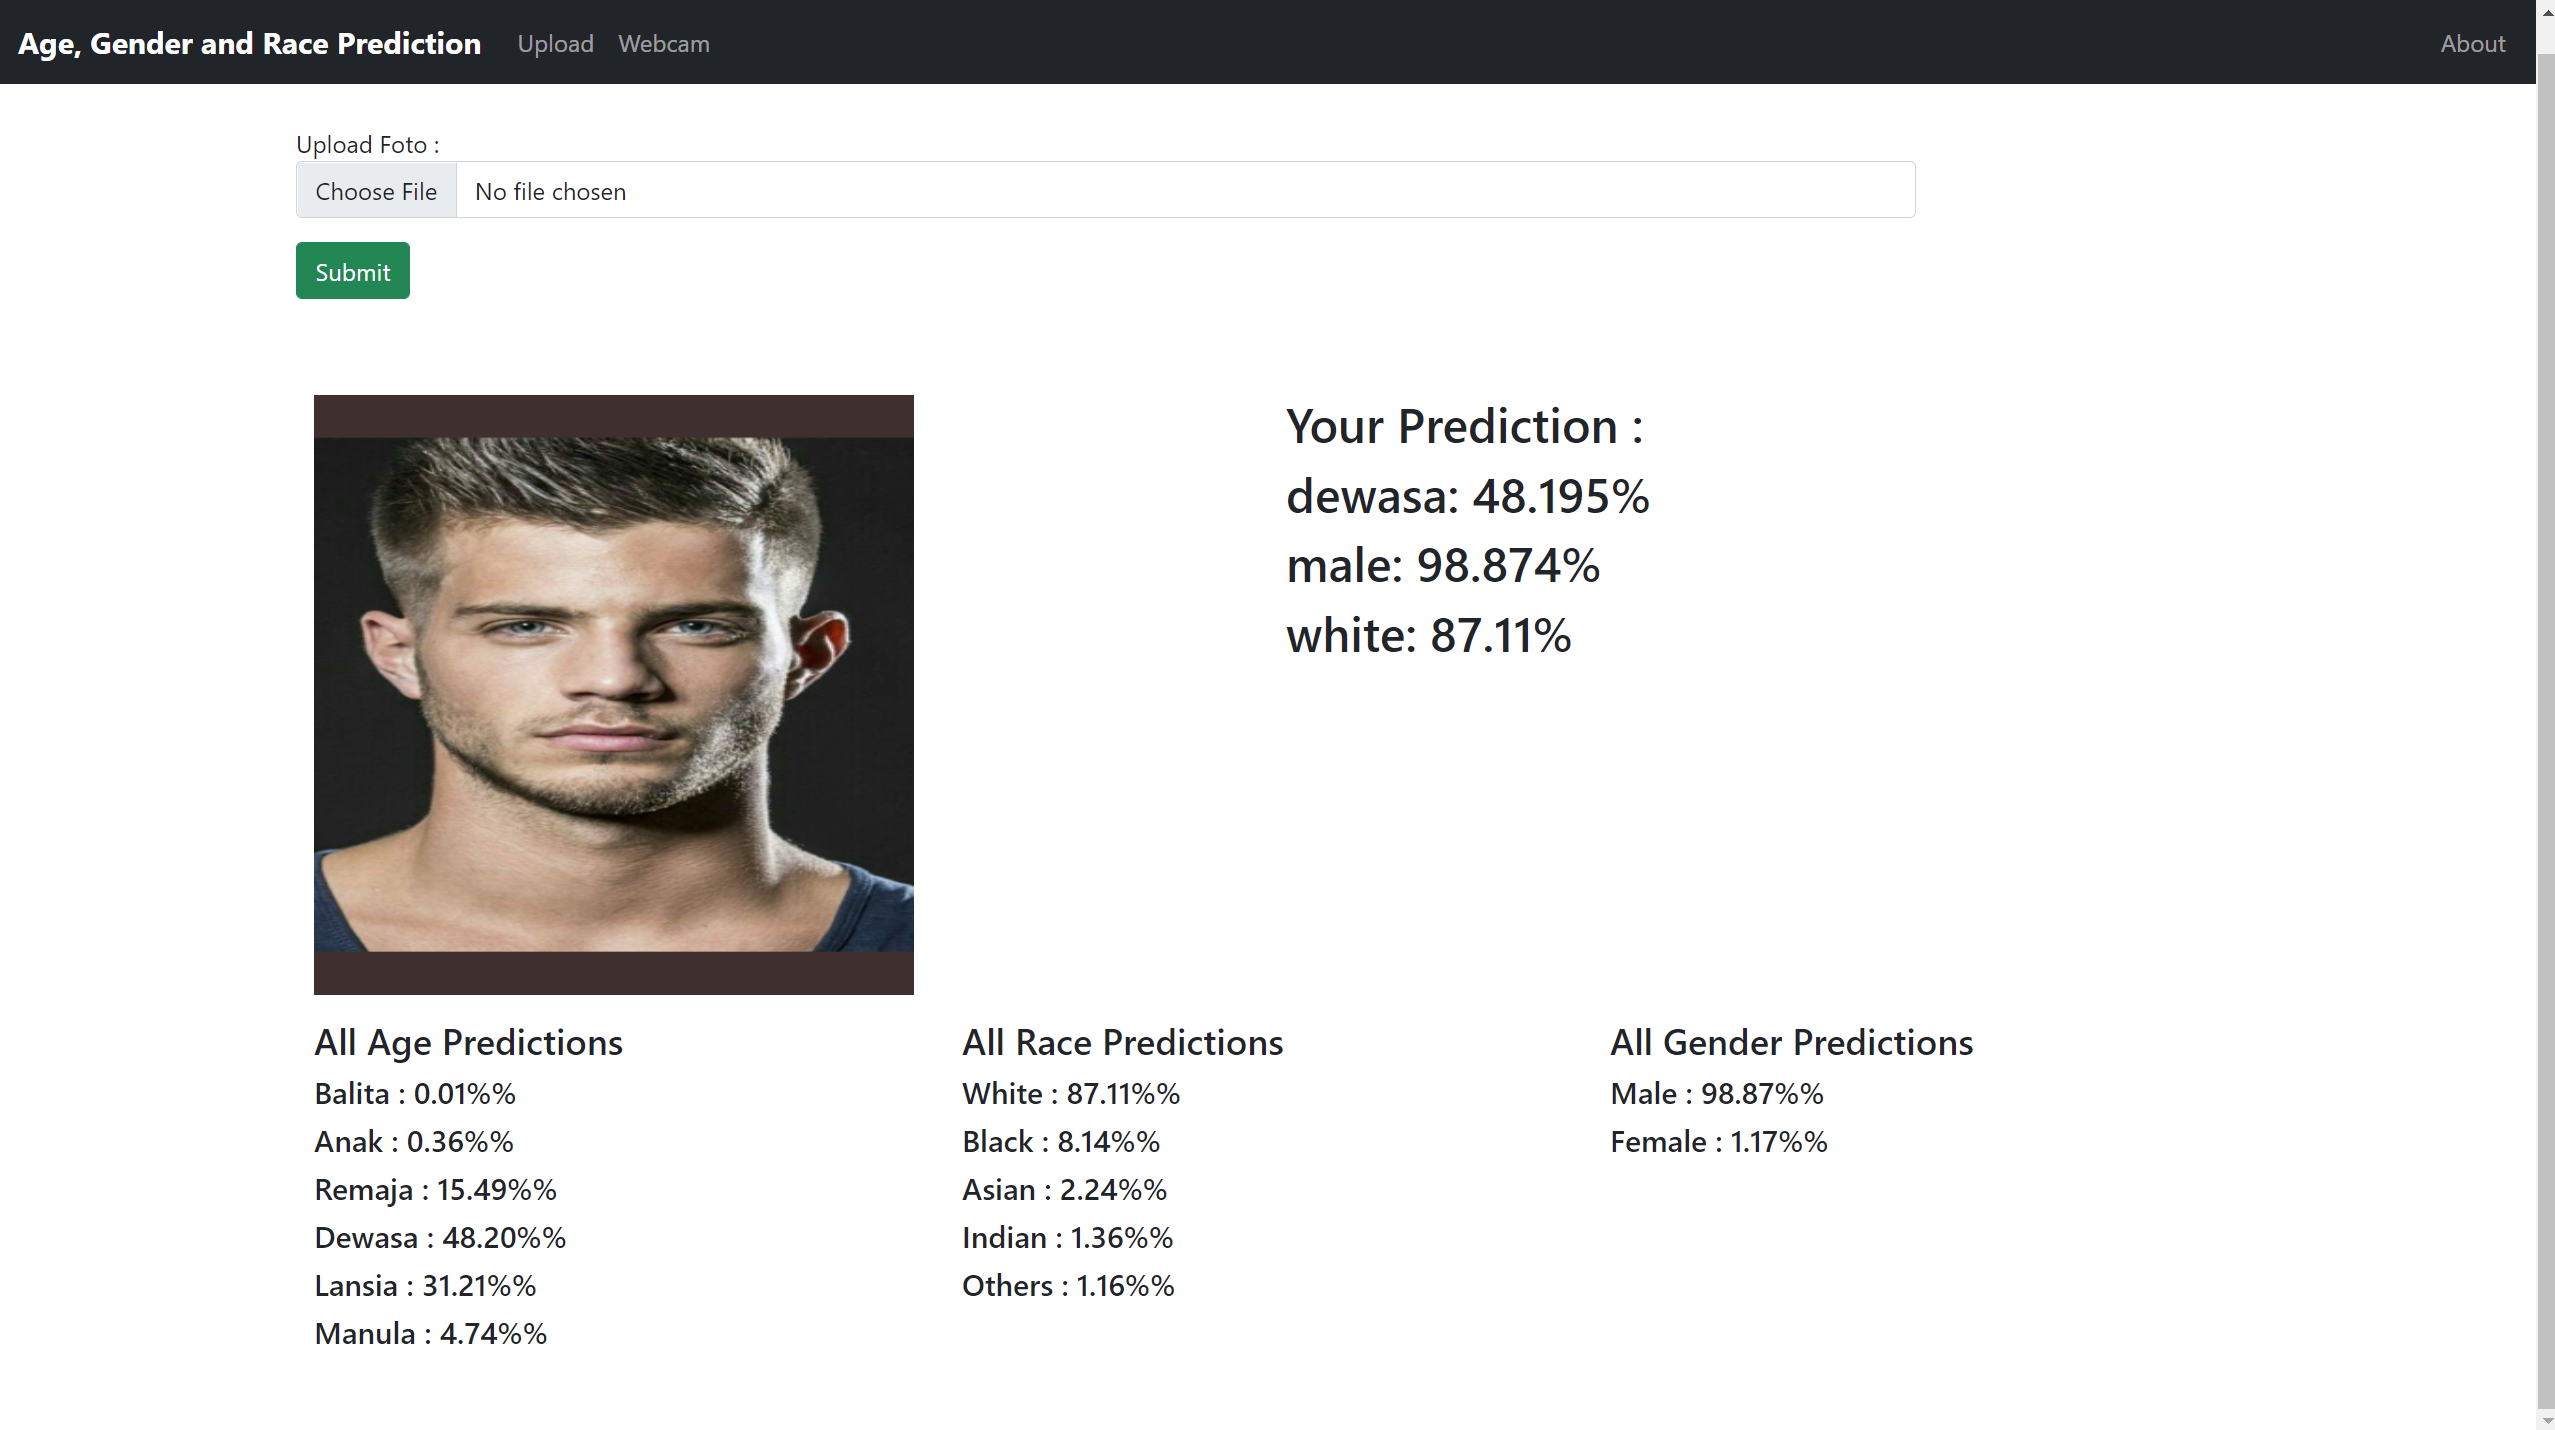
\includegraphics[width=0.4\textwidth]{gambar/web.png}

    % Ubah sesuai dengan keterangan gambar yang diinginkan.
    \caption{Hasil estimasi dengan upload foto}
    \label{fig:upload}
  \end{figure}

  Sedangkan untuk hasil prediksi dari metode foto webcam sebagai berikut pada Gambar\ref{fig:webcam}.

  \begin{figure} [ht]
    \centering
    % Ubah sesuai dengan nama file gambar dan ukuran yang akan digunakan.
    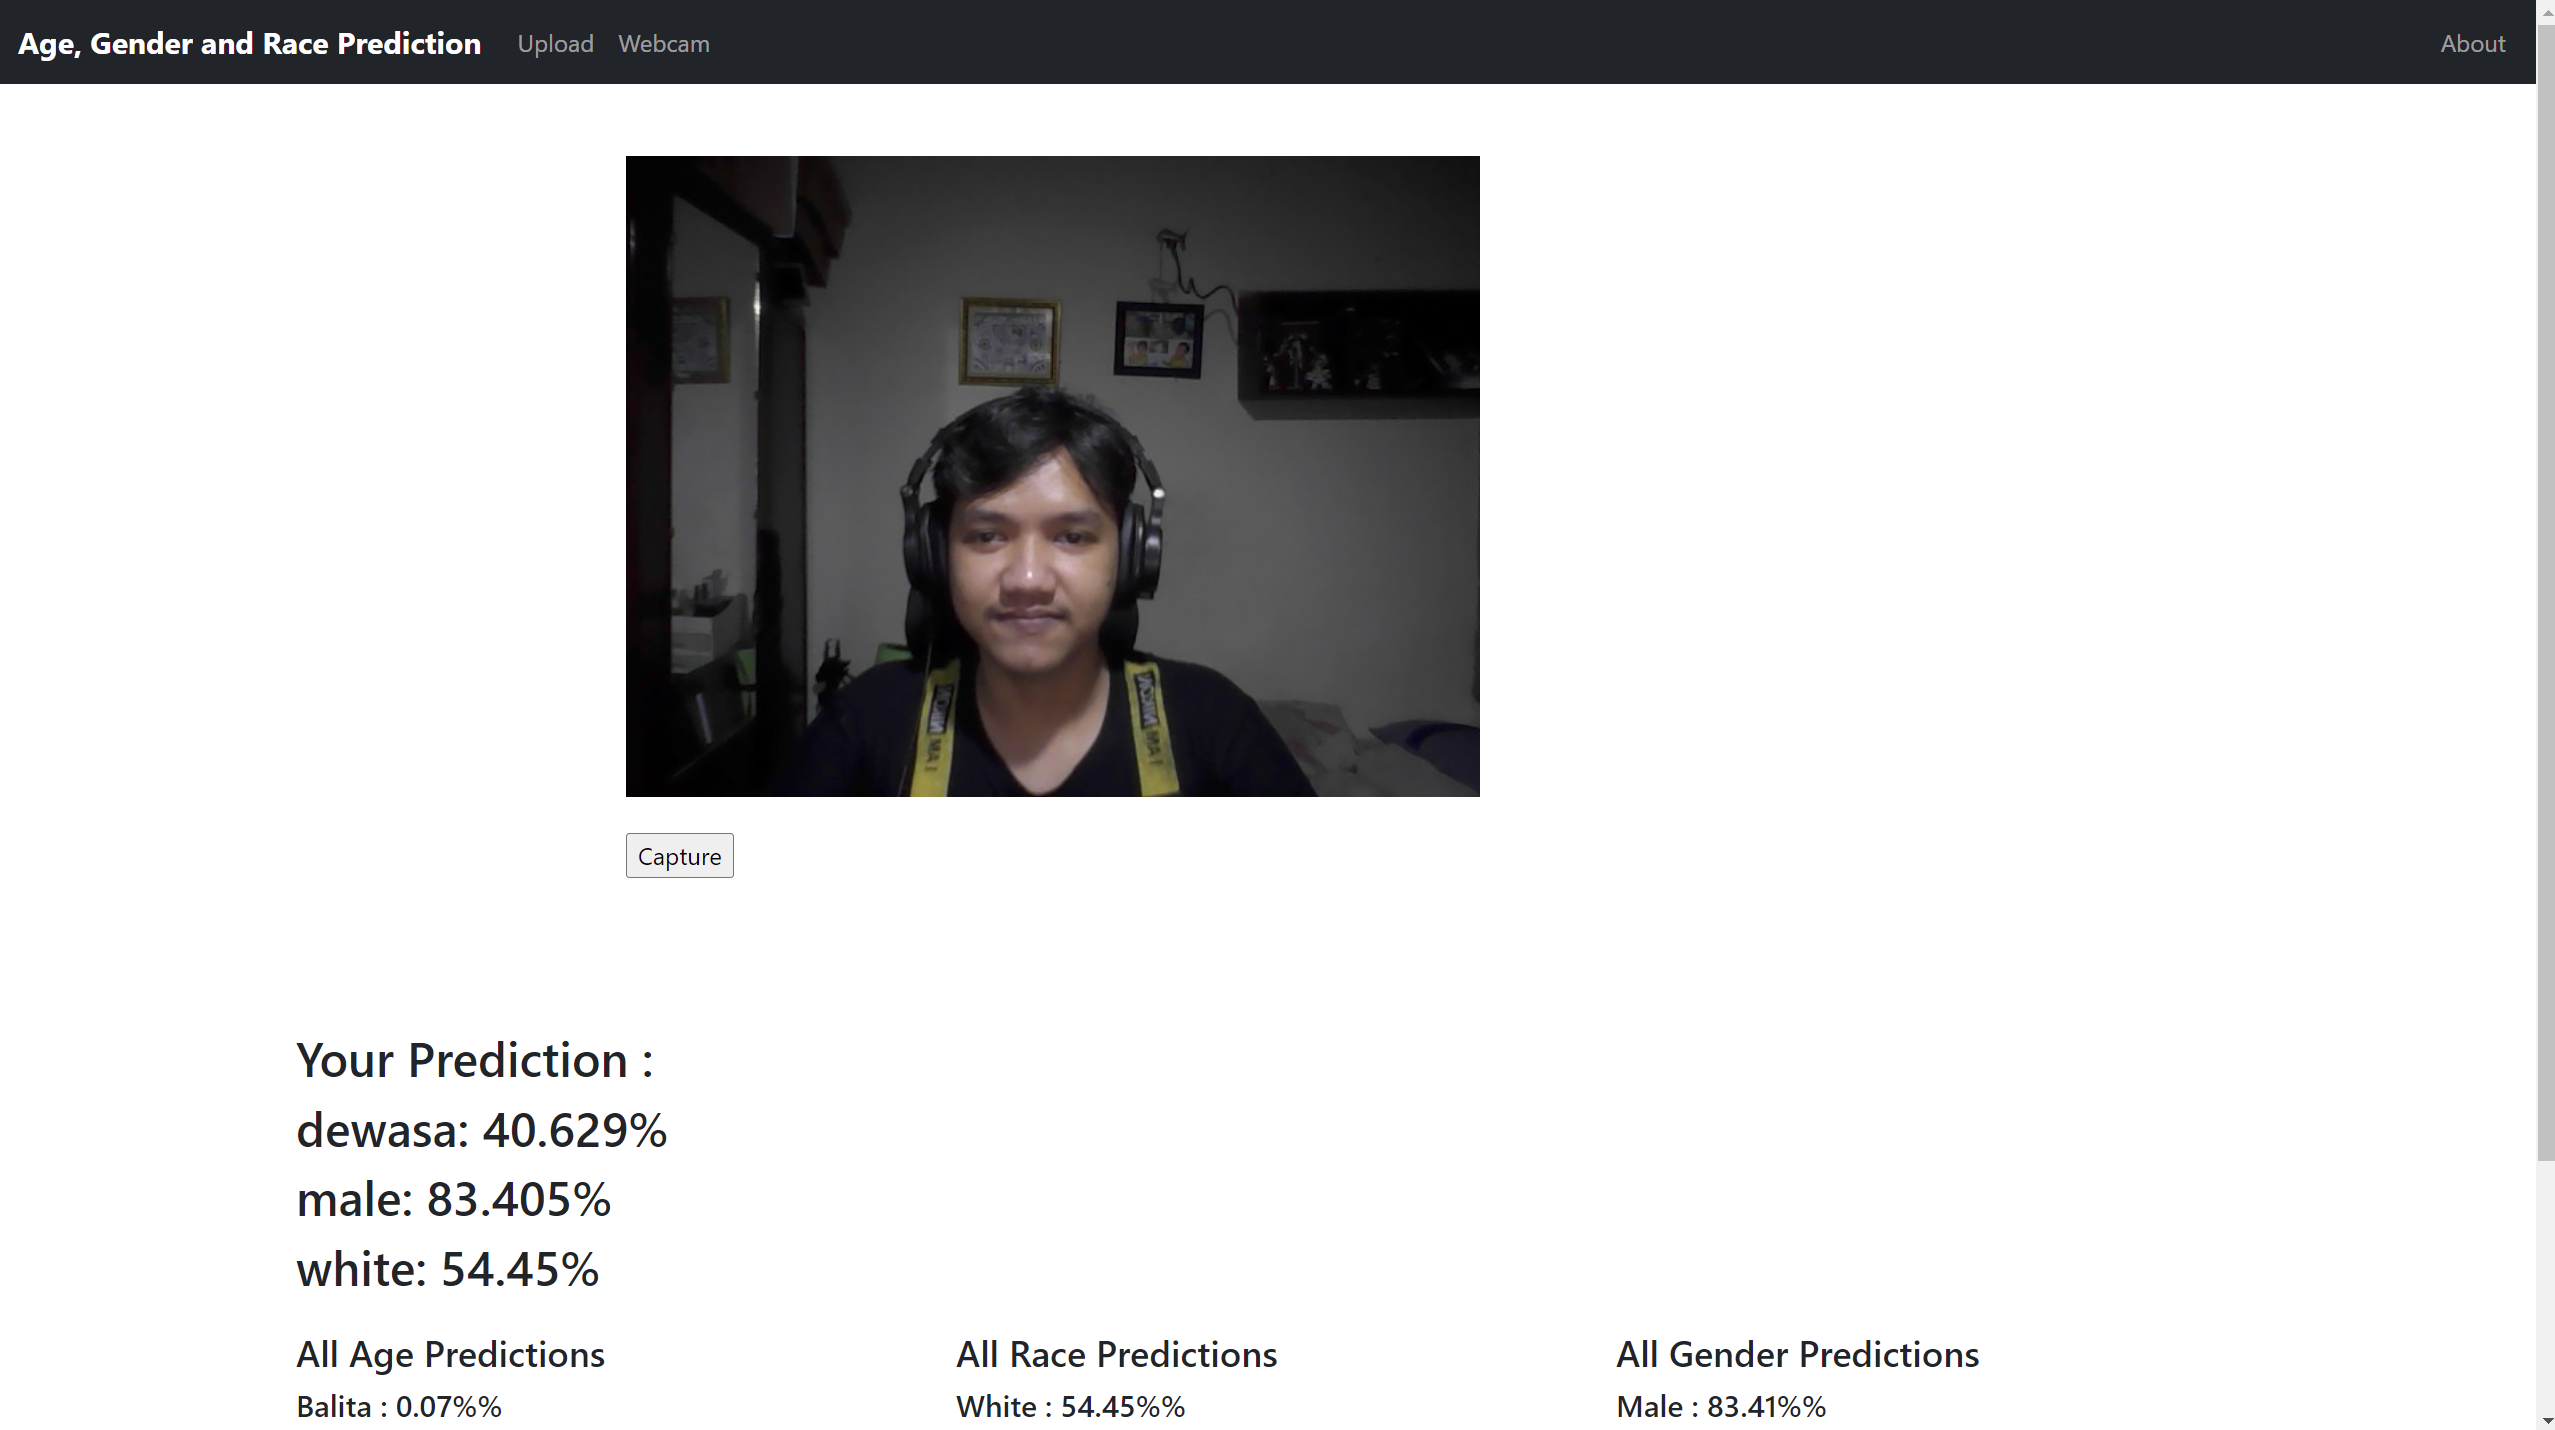
\includegraphics[width=0.4\textwidth]{gambar/web2.png}

    % Ubah sesuai dengan keterangan gambar yang diinginkan.
    \caption{Hasil estimasi dengan foto webcam}
    \label{fig:webcam}
  \end{figure}

\end{enumerate}